\documentclass[9pt]{extarticle}
\title{}
\author{Avinash Iyer}
\date{}
\usepackage[shortlabels]{enumitem}

%font setup
%
%\usepackage[math]{anttor}

%paper setup
\usepackage{geometry}
\geometry{letterpaper, portrait, margin=1in}
\usepackage{fancyhdr}

\usepackage{blkarray}
\usepackage{nicematrix}
%symbols
\usepackage{amsmath}
\usepackage{mathtools}
\usepackage{amssymb}
\usepackage{hyperref}
\usepackage{gensymb}

\usepackage[T1]{fontenc}
\usepackage[utf8]{inputenc}

%chemistry stuff
\usepackage[version=4]{mhchem}
\usepackage{chemfig}

%plotting
\usepackage{pgfplots}
\usepackage{tikz}

%\usepackage{natbib}

%graphics stuff
\usepackage{graphicx}
\graphicspath{ {./images/} }

%code stuff
%when using minted, make sure to add the -shell-escape flag
%you can use lstlisting if you don't want to use minted
%\usepackage{minted}
%\usemintedstyle{pastie}
%\newminted[javacode]{java}{frame=lines,framesep=2mm,linenos=true,fontsize=\footnotesize,tabsize=3,autogobble,}
%\newminted[cppcode]{cpp}{frame=lines,framesep=2mm,linenos=true,fontsize=\footnotesize,tabsize=3,autogobble,}

\usepackage{listings}
\usepackage{color}
\definecolor{dkgreen}{rgb}{0,0.6,0}
\definecolor{gray}{rgb}{0.5,0.5,0.5}
\definecolor{mauve}{rgb}{0.58,0,0.82}

\lstset{frame=tb,
	language=Java,
	aboveskip=3mm,
	belowskip=3mm,
	showstringspaces=false,
	columns=flexible,
	basicstyle={\small\ttfamily},
	numbers=none,
	numberstyle=\tiny\color{gray},
	keywordstyle=\color{blue},
	commentstyle=\color{dkgreen},
	stringstyle=\color{mauve},
	breaklines=true,
	breakatwhitespace=true,
	tabsize=3
}
% text + color boxes
\usepackage{tcolorbox}
\tcbuselibrary{breakable}
\newtcolorbox{problem}[1]{colback = white, title = {#1}, breakable}
\newtcolorbox{solution}{colback = white, colframe = black!75!white, title = Solution, breakable}
%including PDFs
\usepackage{pdfpages}
\setlength{\parindent}{0pt}

\pagestyle{fancy}
\fancyhf{}
\rhead{Avinash Iyer}
\lhead{Homework solutions up to Midterm 1}
\begin{document}
\section*{1.1}%
\subsection*{Individual}
\begin{problem}{1.1.1}
  Determine which complete bipartite graphs are complete graphs.
  \tcblower
  $K_{1,1}$ is the only complete bipartite graph that is complete
\end{problem}
\begin{problem}{1.1.3}
  Using rectangular blocks whose entries are all equal, write down an adjacency matrix for $K_{m,n}$.
  \tcblower
  \[
    K_{m,n} = \begin{bNiceMatrix}[first-row,first-col]
          & a_1 & a_2 & \cdots & a_m & b_1 & b_2 & \cdots & b_n \\
      a_1 & 0 & 0 & \cdots & 0 & 1 & 1 & \cdots & 1 \\
      a_2 & 0 & 0 & \cdots & 0 & 1 & 1 & \cdots & 1 \\
      \vdots & \vdots & \vdots & \ddots & \vdots & \vdots & \ddots & \vdots \\
      a_m & 0 & 0 & \cdots & 0 & 1 & 1 & \cdots & 1 \\
      b_1 & 1 & 1 & \cdots & 1 & 0 & 0 & \cdots & 0 \\
      b_2 & 1 & 1 & \cdots & 1 & 0 & 0 & \cdots & 0 \\
      \vdots & \vdots & \vdots & \ddots & \vdots & \vdots & \ddots & \vdots \\
      b_n & 1 & 1 & \cdots & 1 & 0 & 0 & \cdots & 0 \\
    \end{bNiceMatrix}
  \]
\end{problem}
\begin{problem}{1.1.5}
    Prove or disprove: If every vertex of a simple graph $G$ has degree 2, then $G$ is a cycle.
    \tcblower
  Let $G$ be the following graph:
    \begin{center}
        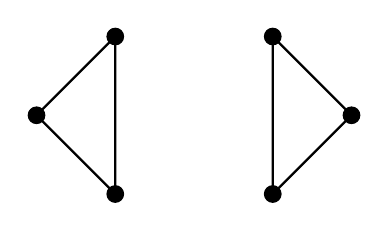
\begin{tikzpicture}
          \draw[fill = black] (1,1) circle (3pt);
          \draw[fill = black] (1,-1) circle (3pt);
          \draw[fill = black] (2,0) circle (3pt);

          \draw[fill = black] (-2,0) circle (3pt);
          \draw[fill = black] (-1,1) circle (3pt);
          \draw[fill = black] (-1,-1) circle (3pt);

        \draw[thick] (1,1) -- (1,-1) -- (2,0) -- (1,1);
        \draw[thick] (-1,1) -- (-1,-1) -- (-2,0) -- (-1,1);
        \end{tikzpicture}
    \end{center}
    Every vertex in $G$ has a degree 2, yet $G$ is not a cycle. 
\end{problem}
\begin{problem}{1.1.8}
    Prove that the 8 vertex graph below decomposes into copies of $K_{1,3}$ and also into copies of $P_4$
  \begin{center}
      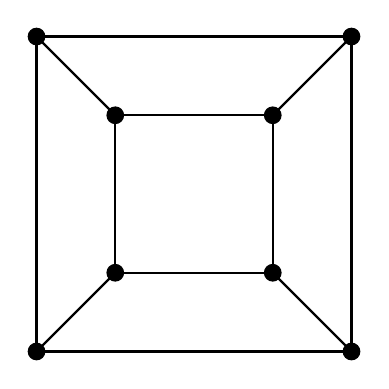
\begin{tikzpicture}
        \draw[fill=black] (1,1) circle (3pt);
        \draw[fill=black] (-1,1) circle (3pt);
        \draw[fill=black] (-1,-1) circle (3pt);
        \draw[fill=black] (1,-1) circle (3pt);

        \draw[fill=black] (2,2) circle (3pt);
        \draw[fill=black] (-2,2) circle (3pt);
        \draw[fill=black] (-2,-2) circle (3pt);
        \draw[fill=black] (2,-2) circle (3pt);
        
        \draw[thick] (1,1) -- (-1,1) -- (-1,-1) -- (1,-1) -- (1,1);
        \draw[thick] (2,2) -- (-2,2) -- (-2,-2) -- (2,-2) -- (2,2);
        \draw[thick] (1,1) -- (2,2);
        \draw[thick] (-1,1) -- (-2,2);
        \draw[thick] (-1,-1) -- (-2,-2);
        \draw[thick] (1,-1) -- (2,-2);
      \end{tikzpicture}
  \end{center} 
  \tcblower
    \begin{center}
      \includegraphics[width=10cm]{1_1_8}
    \end{center}
\end{problem}
\begin{problem}{1.1.9}
      Prove that the graph below is isomorphic to the complement of the previous graph
  \begin{center}
      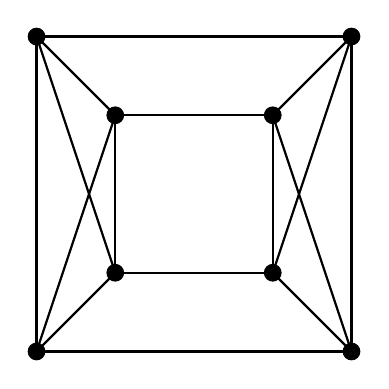
\begin{tikzpicture}
        \draw[fill=black] (1,1) circle (3pt);
        \draw[fill=black] (-1,1) circle (3pt);
        \draw[fill=black] (-1,-1) circle (3pt);
        \draw[fill=black] (1,-1) circle (3pt);

        \draw[fill=black] (2,2) circle (3pt);
        \draw[fill=black] (-2,2) circle (3pt);
        \draw[fill=black] (-2,-2) circle (3pt);
        \draw[fill=black] (2,-2) circle (3pt);
        
        \draw[thick] (1,1) -- (-1,1) -- (-1,-1) -- (1,-1) -- (1,1);
        \draw[thick] (2,2) -- (-2,2) -- (-2,-2) -- (2,-2) -- (2,2);
        \draw[thick] (1,1) -- (2,2);
        \draw[thick] (-1,1) -- (-2,2);
        \draw[thick] (-1,-1) -- (-2,-2);
        \draw[thick] (1,-1) -- (2,-2);
        \draw[thick] (2,2) -- (1,-1);
        \draw[thick] (2,-2) -- (1,1);
        \draw[thick] (-2,2) -- (-1,-1);
        \draw[thick] (-2,-2) -- (-1,1);
      \end{tikzpicture}
  \end{center} 
  \tcblower
  \begin{center}
    \includegraphics[width=10cm]{1_1_9}
  \end{center}
\end{problem}
\begin{problem}{1.1.10}
   Prove or disprove: the complement of a simple disconnected graph must be connected.
   \tcblower
   Let $G$ be a graph that is disconnected. We want to show that $\forall x,y\in V(G), \exists xz$ path. We can split into two cases.
     \begin{itemize}
       \item Suppose $x\not\leftrightarrow y$ in $G$. Then, in $\overline{G}$, $x\leftrightarrow y$ by the definition of a graph complement.
       \item Suppose $x\leftrightarrow y$ in $G$. Then, since $G$ is disconnected, we know that there must be some $z\in V(G)$ such that there is no $xz$ path. Since there is no $xz$ path, then there is no $yz$ path. In particular, this means $x\not\leftrightarrow z$ and $y\not\leftrightarrow z$ in $G$. Therefore, in $\overline{G}$, we have that $x\leftrightarrow z$ and $y\leftrightarrow z$, meaning there is a path between $x$ and $y$.
     \end{itemize}
\end{problem}
\subsection*{Group}%
\begin{problem}{1.1.13}
    Let $G$ be the graph whose vertex set is the set of $k$-tuples with coordinates $\{0,1\}$, with $x$ adjacent to $y$ if $x$ and $y$ differ by exactly one position. Determine whether $G$ is bipartite.
    \tcblower
  $G$ is bipartite --- we can find a bipartition by separating the set into a set of tuples which differ by an even number of positions and a set of tuples which differ by an odd number of positions. Since odd numbers differ from each other by at least $2$ places, and even numbers differ from each other by at least $2$ places, we know that each subset of tuples is not adjacent to each other, but is adjacent to the other set. 
\end{problem}
\begin{problem}{1.1.26}
  Let $G$ be a graph with girth $4$ in which every vertex has degree $k$. Prove that $G$ has at least $2k$ vertices. Determine all such graphs with $2k$ vertices.
  \tcblower
  \noindent Suppose $G$ is a graph with girth $4$ with every vertex of degree $k$. Let $v_i\in V(G)$. Then, there must be $k$ vertices which $v_i$ is adjacent to. However, none of these vertices can be adjacent to themselves or $G$ would have girth $3$. Thus, we can form a bipartition such that $v_i$ is in a set of at least $k$ vertices such that each vertex is not adjacent to itself, and each vertex in this set is adjacent to $k$ vertices in a disjoint set where each vertex in this set is not adjacent to any other vertex in this set. Therefore, there are at least $2k$ vertices.\\

  \noindent The graphs with exactly $2k$ vertices are the $K_{n,n}$ complete bipartite graphs.
\end{problem}
\begin{problem}{1.1.27}
  Let $G$ be a graph with girth 5. Prove that if every vertex of $G$ has degree at least $k$, then $G$ has at least $k^2+1$ vertices. For $k=2$ and $k=3$, find one such graph with $k^2+1$ vertices.
  \tcblower
  Let $G$ be a simple graph with girth 5. Suppose that every vertex of $G$ has degree $k$. Let $u\in V(G)$. Then, $u$ has $k$ adjacent vertices, each of which is not adjacent to each other (or else the girth of $G$ would be $3$). Let this set be $N$. The elements of $N$ cannot have any other common neighbors aside from $u$, or else the girth of $G$ would be $4$, meaning each has $k-1$ distinct neighbors. Therefore, the total number of vertices in our graph includes $u$, the elements of $N$ that are the $k$ distinct neighbors of $u$, and the $k(k-1)$ distinct vertices for each vertex in $N$. Therefore, our total is $1 + k + k(k-1) = k^2 + 1$.\\

  If there were any vertex with degree greater than $k$, then there would be additional vertices beyond the $k^2 + 1$ vertices necessary for a $k$-regular graph.\\

  For  $k=2$, we have the graph $C_5$ for an example of a graph with $k^2 + 1$ vertices, and for $k=3$ we have the Petersen graph.
\end{problem}
\begin{problem}{1.1.30}
    Let $G$ be a simple graph with adjacency matrix $A$ and incidence matrix $M$. Prove that the degree of $v_i$ is the $i$th diagonal entry of $A^2$ and $MM^T$. What do the entries in position $(i,j)$ of $A^2$ and $MM^T$ say about $G$?
\tcblower
  Let $A$ be the adjacency matrix for a simple graph $G$. In $A$, every vertex's corresponding row and column are identical, meaning that the entry $A^2_{i,i}$ will be equal to $r_ic_i$ for row $i$ and column $i$ corresponding to $v_i$. Thus, $r_ic_i$ is equal to $|c_i|^2$, which is equal to the sum of the elements of $c_i$, which is equal to the degree of $v_i$.\\

  Let $M$ be the incidence matrix for a simple graph $G$. In $MM^T$, the diagonal element $MM^T_{i,i}$ will be equal to $r_i r_i^T$, where $r_i$ represents the edge incidence row of $v_i$. This is equal to $\left|r_i^T\right|^2$, which is equal to the sum of the elements of $r_i$, which is equal to the number of edges incident on $v_i$, which is equal to the degree of $v_i$.\\

  The entry in position $(i,j)$ in both $A^2$ and $MM^T$ shows whether vertices $v_i$ and $v_j$ are adjacent to each other.
\end{problem}
\begin{problem}{1.1.34}
    Decompose the Petersen graph into three connected subgraphs that are pairwise isomorphic. Also decompose it into copies of $P_4$.
    \tcblower
  \begin{center}
    \includegraphics[width = 15cm]{1_1_34.pdf}
  \end{center}
\end{problem}
\section*{1.2}%
\subsection*{Individual}%
\begin{problem}{1.2.1}
    Determine whether the following statements are true or false:
      \begin{itemize}
        \item Every disconnected graph has an isolated vertex.
        \item A graph is connected if and only if some vertex is connected to all other vertices.
        \item The edge set of every closed trail can be partitioned into edge sets of cycles.
        \item If a maximal trail in a graph is not closed, then its endpoints have odd degree.
      \end{itemize}
      \tcblower
      \begin{itemize}
        \item False; we can imagine a graph with two components, each of which consists of $K_3$, where there are no isolated vertices.
        \item True; since $\forall u,v\in G,\exists u,v$ path by the definition of a connected graph, this means any vertex must have a path to any other vertex.
        \item True; every closed trail contains within it a cycle --- we can delete the edge set of this cycle, and find cycles within remaining components until we reach isolated vertices.
        \item True; if there were a maximal trail with an endpoint of even degree, then we would be able to extend the trail further by re-entering the endpoint vertex.
      \end{itemize}
\end{problem}
\begin{problem}{1.2.5}
  Let $v$ be a vertex of a connected simple graph $G$. Prove that $v$ has a neighbor in every component of $G-v$. Explain why this allows us to conclude that no graph has a cut-vertex of degree 1.   
  \tcblower
  Suppose that $G-v$ is connected. Then, since $G$ is connected, and $v\in V(G)$, it must be the case that $v$ is connected to every component of $G-v$, meaning that it has a neighbor in every component of $G-v$ as $G-v$ is connected.\\

  Now suppose that $G-v$ is disconnected, meaning that it has more than one component after removing $v$. Before, $v$ must have been connected to every vertex in $G$ as $G$ was a simple connected graph, and afterwards $G-v$ is no longer connected, meaning that $v$ is a cut-vertex. This means $v$ must have been adjacent to a vertex in each component of $G-v$, as removing the incident edges on $v$ along with $v$ increased the number of components from the original $1$ that was in $G$.\\

  From this result, we can conclude that no cut-vertex has degree $1$ as removing a vertex of degree $1$ and its incident edges does not increase the number of components in $G$, since there is only one edge incident on a vertex of degree $1$.
\end{problem}
\begin{problem}{1.2.6}
  In the graph below, find all the maximal paths, maximal cliques, and maximal independent sets. Also, find all the maximum paths, cliques, and independent sets. 
    \begin{center}
        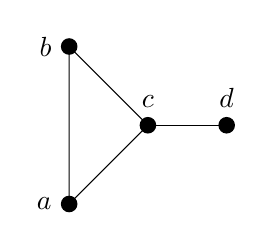
\begin{tikzpicture}
          \fill (0,0) circle (3pt);
          \fill (-1,1) circle (3pt);
          \fill (-1,-1) circle (3pt);
          \fill (1,0) circle (3pt);
          \node[anchor = south] at (0,0.1) {$c$};
          \node[anchor = south] at (1,0.1) {$d$};
          \node[anchor = east] at (-1.1,-1) {$a$};
          \node[anchor = east] at (-1.1,1) {$b$};
          \draw (-1,-1) -- (-1,1) -- (0,0) -- (-1,-1);
          \draw (0,0) -- (1,0);
        \end{tikzpicture}
    \end{center}
    \tcblower
  \begin{itemize}
      \item The maximal paths are as follows:
     \begin{itemize}
       \item $d,c,b,a$
       \item $d,c,a,b$
       \item $a,b,c,d$
       \item $b,a,c,d$
       \item $b,c,a$
       \item $c,b,a$
       \item $a,c,b$
     \end{itemize}
   \item The maximal cliques are $K_3$ consisting of $a,b,c$ and $K_2$ consisting of $c,d$.
   \item The maximal independent sets are $\{a,d\}$ and  $\{b,d\}$.
   \item The maximum path is any of those paths listed above with length $4$.
   \item The maximum clique is $K_3$.
   \item The maximum independent sets are those listed above with size $2$.
  \end{itemize}
\end{problem}
\begin{problem}{1.2.8}
  Determine the values of $m$ and $n$ such that $K_{m,n}$ is Eulerian. 
  \tcblower
  \[
    m,n\in 2\mathbb{Z}^{+}
  \]
\end{problem}
\begin{problem}{1.2.10}
  Prove or disprove:
  \begin{enumerate}[(a)]
      \item Every Eulerian bipartite graph has an even number of edges.
      \item Every Eulerian simple graph with an even number of vertices has an even number of edges.
    \end{enumerate}
    \tcblower
  \begin{tcolorbox}[colback = white, title = (a)]
    Let $G$ be an Eulerian bipartite graph. Since $G$ is Eulerian, it must contain an Eulerian cycle, meaning that as seen above, there are an even number of vertices, meaning that there are an even number of edges in $G$. 
  \end{tcolorbox}

  \begin{tcolorbox}[colback = white, title = (b)]
    Let $G$ be an Eulerian simple graph with an even number of vertices. Since $G$ is Eulerian, this means there must be an Eulerian circuit $C$ that traverses every edge exactly once in $G$. Every vertex in $G$ must have even degree (or else we would require a backtrack in our Eulerian cycle, which is not a circuit); a simple pairing of the vertices would yield that we have $\lfloor n/2\rfloor $ edges, and to complete the cycle we need $2(n/2) + 2k$ edges for $n$ vertices and some integer $k$. Therefore, there must be an even number of edges.
  \end{tcolorbox}
\end{problem}
\subsection*{Group}%
\begin{problem}{1.2.20}
  Let $v$ be a cut-vertex of a simple graph $G$. Prove that $\overline{G} - v$ is connected.
  \tcblower
  Let $x,y,v\in V(\overline{G})$, where $v$ is a cut-vertex of $G$.\\

  Suppose $x$ and $y$ belong to distinct components of $G-v$. Then, $xy\not\in E(G)$, meaning that $xy\in E(\overline{G})$, meaning there is an $x,y$ path in $\overline{G}$, so there is an $x,y$ path in $\overline{G}-v$.\\

  Suppose $x$ and $y$ are in the same component of $G-v$. Since $v$ is a cut-vertex, this means there must be at least two components in $G-v$. Let $H_1$ be the component that $x,y$ are in, while $\exists w\in H_2$ is a vertex in $H_2$ disjoint from $H_1$. Since $H_1$ and $H_2$ are disjoint, this means the components do not contain any edges between them, so $x\not\leftrightarrow w$ and $y\not\leftrightarrow w$ in $G-v$ --- however, this means that $x\leftrightarrow w$ and $y\leftrightarrow w$ in $\overline{G}$, meaning that $\exists x,y$ path in $\overline{G} - v$.
\end{problem}
\begin{problem}{1.2.22}
  Prove that a graph is connected if and only if for every partition of its vertices into two nonempty sets, there is an edge with endpoints in both sets. 
  \tcblower
  Let $G$ be a graph where there exists a partition of its vertices into two non-empty sets such that there is no edge with endpoints in both sets. Call these sets $A$ and $B$. By our assumptions, $\forall u\in A$ and $\forall v\in B$, $\nexists e$ such that $e = uv$. Therefore, we cannot create a path between any $u\in A$ and any $v\in B$ as there is no edge to connect any element in $A$ and any element in $B$. Therefore, $G$ is disconnected.\\

  Suppose $G$ is a disconnected graph. Then, $G$ contains more than one component --- we can create a partition of $V(G)$ by letting $H_1,H_2,\dots,H_k$ refer to the $k$ components of $G$. Each of these components is necessarily disjoint from every other component. By taking $H = H_1\cup H_2\cup\dots\cup H_{k-1}$ as one set and $H_k$ as our other set, we know that $H_1,\dots,H_k$ are all disjoint, meaning that $H$ and $H_k$ are disjoint, meaning that there is no edge connecting any vertex $H$ with any vertex in $H_k$, meaning we have created a partition of $G$ such that there exists no edge between any vertex in one set and any vertex in the other set.
\end{problem}
\begin{problem}{1.2.26}
  Prove that a graph $G$ is bipartite if and only if every subgraph $H$ of $G$ has an independent set consisting of at least half of $V(H)$.
  \tcblower
  Suppose $G$ is bipartite. Then, there exists a partition of the vertices $V = X\sqcup Y$ such that $X$ and $Y$ are independent sets. Let $H$ be a subgraph of $G$, and let $H_X = X\cap V(H)$ and $H_Y = Y\cap H$. Because $H$ is a subgraph of $G$, each vertex of $H$ must be an element of either $H_X$ or $H_Y$, or that $V(H) = H_X \sqcup H_Y$. WLOG, let $|H_X|>|H_Y|$. Since $H_X\subseteq X$ and $X$ is an independent set, $H_X$ is an independent subset consisting of at least half of $V(H)$.\\

  Suppose every subgraph of $G$ has an independent set consisting of at least half of $V(H)$. We will suppose toward contradiction that $G$ is not bipartite. Then, $G$ must contain an odd cycle, $H_1$. However, an independent set of $H_1$ consists of at most $\left\lfloor \frac{|V(H_1)|}{2}\right\rfloor < \frac{|V(H_1)|}{2}$, otherwise two vertices would be adjacent. Because $H_1$ is an independent set with less than half of the elements of $V(H)$, we have reached a contradiction. Therefore, $G$ must be bipartite.
\end{problem}
\begin{problem}{1.2.38}
  Prove that every $n$-vertex graph with at least $n$ edges contains a cycle.
  \tcblower
  We proceed via induction as follows:\\

  For the base case where $|V(G)| = 1$, we know that there is a cycle with one edge that connects back on the vertex.\\

  For the case where $|V(G)| > 1$, if $v\in V(G)$ has degree at most $1$, then $G-v$ has $n-1$ vertices and at least $n-1$ edges, so by our inductive hypothesis, we know that $G-v$ contains a cycle. Meanwhile, if $\forall v\in V(G), d(v)\geq 2$, we know by Lemma 1.2.25 that $G$ contains a cycle.
\end{problem}
\section*{1.3}%
\subsection*{Individual}%
  \begin{problem}{1.3.3}
    Let $u$ and $v$ be adjacent vertices in $G$. Prove that $uv$ belongs to at least $d(u) + d(v) - n(G)$ triangles in $G$.
  \tcblower
    Let $u\leftrightarrow v \in G$. In order for $uv$ to be in a triangle in $G$, $u$ and $v$ must share a common neighbor. By using the property of inclusion and exclusion, we can find the set as follows:
    \begin{align*}
      |N(u) \cup N(v)| &= |N(u)| + |N(v)| - |N(u) \cap N(v)| \\
      |N(u) \cap N(v)| &= |N(u)| + |N(v)| - |N(u) \cup N(v)| \\
                       &\geq d(u) + d(v) - n(G)
    \end{align*}
  \end{problem}
  \begin{problem}{1.3.4}
    Prove that the graph below is isomorphic to $Q_4$.
    \begin{center}
      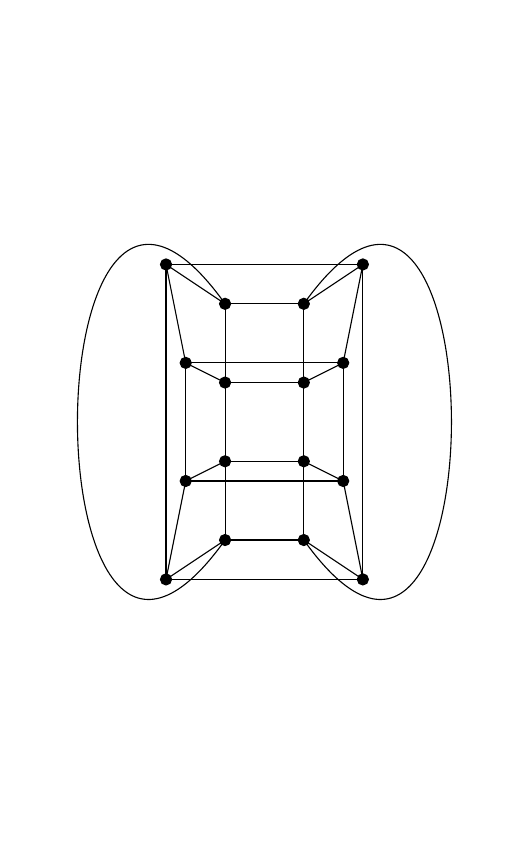
\begin{tikzpicture}
        % \draw[thin, gray] (-3,-3) grid (3,3);
        % drawing points
        \filldraw (0.5,0.5) circle (2pt);
        \filldraw (-0.5,0.5) circle (2pt);
        \filldraw (0.5,-0.5) circle (2pt);
        \filldraw (-0.5,-0.5) circle (2pt);
        \filldraw (1,0.75) circle (2pt);
        \filldraw (-1,0.75) circle (2pt);
        \filldraw (-1,-0.75) circle (2pt);
        \filldraw (1,-0.75) circle (2pt);
        \filldraw (0.5,1.5) circle (2pt);
        \filldraw (-0.5,1.5) circle (2pt);
        \filldraw (-0.5,-1.5) circle (2pt);
        \filldraw (0.5,-1.5) circle (2pt);
        \filldraw (1.25,2) circle (2pt);
        \filldraw (-1.25,2) circle (2pt);
        \filldraw (1.25,-2) circle (2pt);
        \filldraw (-1.25,-2) circle (2pt);
        % drawing lines
        \draw (0.5,0.5) -- (-0.5,0.5) -- (-0.5,-0.5) -- (0.5,-0.5) -- (0.5,0.5);
        \draw (-1.25,-2) -- (1.25,-2) -- (1.25,2) -- (-1.25,2) -- (-1.25,-2);
        \draw (1,0.75) -- (-1,0.75) -- (-1,-0.75) -- (1,-0.75) -- (1,0.75);
        \draw (0.5,1.5) -- (0.5,0.5);
        \draw (-0.5,1.5) -- (-0.5,0.5);
        \draw (-0.5,-1.5) -- (-0.5,-0.5);
        \draw (0.5,-1.5) -- (0.5,-0.5);
        \draw (0.5,-1.5) -- (-0.5,-1.5);
        \draw (0.5,1.5) -- (-0.5,1.5);
        \draw (1.25,2) -- (0.5,1.5);
        \draw (-1.25,2) -- (-0.5,1.5);
        \draw (-1.25,-2) -- (-0.5,-1.5);
        \draw (1.25,-2) -- (0.5,-1.5);
        \draw (1,0.75) -- (1.25,2);
        \draw (-1,0.75) -- (-1.25,2);
        \draw (-1,-0.75) -- (-1.25,-2);
        \draw (1,-0.75) -- (1.25,-2);
        \draw (1,0.75) -- (0.5,0.5);
        \draw (1,-0.75) -- (0.5,-0.5);
        \draw (-1,-0.75) -- (-0.5,-0.5);
        \draw (-1,0.75) -- (-0.5,0.5);
        \draw (0.5,1.5) .. controls (3,5) and (3,-5) .. (0.5,-1.5);
        \draw (-0.5,1.5) .. controls (-3,5) and (-3,-5) .. (-0.5,-1.5);
      \end{tikzpicture} 
    \end{center}
  \tcblower
    We can assign tuples to the graph as follows:
    \begin{center}

      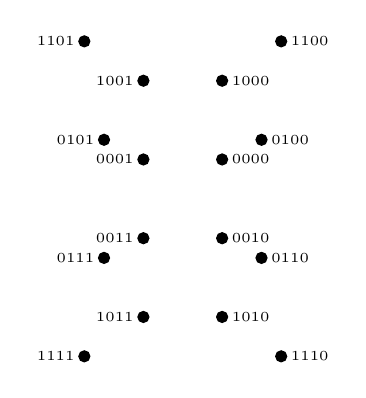
\begin{tikzpicture}
        % \draw[thin, gray] (-3,-3) grid (3,3);
        % drawing points
        \filldraw (0.5,0.5) circle (2pt);
        \node [anchor = west] at (0.5,0.5) {\tiny $0000$};
        \filldraw (-0.5,0.5) circle (2pt);
        \node [anchor = east] at (-0.5,0.5) {\tiny $0001$};
        \filldraw (0.5,-0.5) circle (2pt);
        \node [anchor = west] at (0.5,-0.5) {\tiny $0010$};
        \filldraw (-0.5,-0.5) circle (2pt);
        \node [anchor = east] at (-0.5,-0.5) {\tiny $0011$};
        \filldraw (1,0.75) circle (2pt);
        \node [anchor = west] at (1,0.75) {\tiny $0100$};
        \filldraw (-1,0.75) circle (2pt);
        \node [anchor = east] at (-1,0.75) {\tiny $0101$};
        \filldraw (-1,-0.75) circle (2pt);
        \node [anchor = east] at (-1,-0.75) {\tiny $0111$};
        \filldraw (1,-0.75) circle (2pt);
        \node [anchor = west] at (1,-0.75) {\tiny $0110$};
        \filldraw (0.5,1.5) circle (2pt);
        \node [anchor = west] at (0.5,1.5) {\tiny $1000$};
        \filldraw (-0.5,1.5) circle (2pt);
        \node [anchor = east] at (-0.5,1.5) {\tiny $1001$};
        \filldraw (-0.5,-1.5) circle (2pt);
        \node [anchor = east] at (-0.5,-1.5) {\tiny $1011$};
        \filldraw (0.5,-1.5) circle (2pt);
        \node [anchor = west] at (0.5,-1.5) {\tiny $1010$};
        \filldraw (1.25,2) circle (2pt);
        \node [anchor = west] at (1.25,2) {\tiny $1100$};
        \filldraw (-1.25,2) circle (2pt);
        \node [anchor = east] at (-1.25,2) {\tiny $1101$};
        \filldraw (1.25,-2) circle (2pt);
        \node [anchor = west] at (1.25,-2) {\tiny $1110$};
        \filldraw (-1.25,-2) circle (2pt);
        \node [anchor = east] at (-1.25,-2) {\tiny $1111$};
      \end{tikzpicture} \\ 
      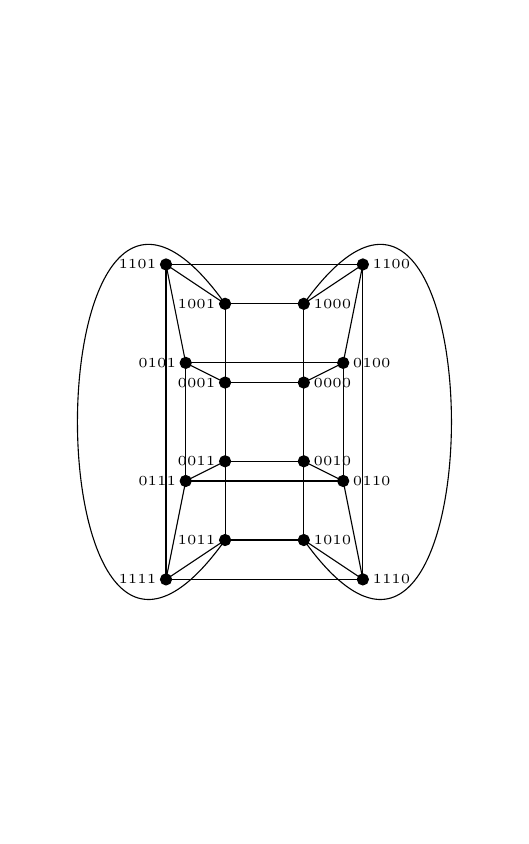
\begin{tikzpicture}
        % \draw[thin, gray] (-3,-3) grid (3,3);
        % drawing points
        \filldraw (0.5,0.5) circle (2pt);
        \node [anchor = west] at (0.5,0.5) {\tiny $0000$};
        \filldraw (-0.5,0.5) circle (2pt);
        \node [anchor = east] at (-0.5,0.5) {\tiny $0001$};
        \filldraw (0.5,-0.5) circle (2pt);
        \node [anchor = west] at (0.5,-0.5) {\tiny $0010$};
        \filldraw (-0.5,-0.5) circle (2pt);
        \node [anchor = east] at (-0.5,-0.5) {\tiny $0011$};
        \filldraw (1,0.75) circle (2pt);
        \node [anchor = west] at (1,0.75) {\tiny $0100$};
        \filldraw (-1,0.75) circle (2pt);
        \node [anchor = east] at (-1,0.75) {\tiny $0101$};
        \filldraw (-1,-0.75) circle (2pt);
        \node [anchor = east] at (-1,-0.75) {\tiny $0111$};
        \filldraw (1,-0.75) circle (2pt);
        \node [anchor = west] at (1,-0.75) {\tiny $0110$};
        \filldraw (0.5,1.5) circle (2pt);
        \node [anchor = west] at (0.5,1.5) {\tiny $1000$};
        \filldraw (-0.5,1.5) circle (2pt);
        \node [anchor = east] at (-0.5,1.5) {\tiny $1001$};
        \filldraw (-0.5,-1.5) circle (2pt);
        \node [anchor = east] at (-0.5,-1.5) {\tiny $1011$};
        \filldraw (0.5,-1.5) circle (2pt);
        \node [anchor = west] at (0.5,-1.5) {\tiny $1010$};
        \filldraw (1.25,2) circle (2pt);
        \node [anchor = west] at (1.25,2) {\tiny $1100$};
        \filldraw (-1.25,2) circle (2pt);
        \node [anchor = east] at (-1.25,2) {\tiny $1101$};
        \filldraw (1.25,-2) circle (2pt);
        \node [anchor = west] at (1.25,-2) {\tiny $1110$};
        \filldraw (-1.25,-2) circle (2pt);
        \node [anchor = east] at (-1.25,-2) {\tiny $1111$};
        % drawing lines
        \draw (0.5,0.5) -- (-0.5,0.5) -- (-0.5,-0.5) -- (0.5,-0.5) -- (0.5,0.5);
        \draw (-1.25,-2) -- (1.25,-2) -- (1.25,2) -- (-1.25,2) -- (-1.25,-2);
        \draw (1,0.75) -- (-1,0.75) -- (-1,-0.75) -- (1,-0.75) -- (1,0.75);
        \draw (0.5,1.5) -- (0.5,0.5);
        \draw (-0.5,1.5) -- (-0.5,0.5);
        \draw (-0.5,-1.5) -- (-0.5,-0.5);
        \draw (0.5,-1.5) -- (0.5,-0.5);
        \draw (0.5,-1.5) -- (-0.5,-1.5);
        \draw (0.5,1.5) -- (-0.5,1.5);
        \draw (1.25,2) -- (0.5,1.5);
        \draw (-1.25,2) -- (-0.5,1.5);
        \draw (-1.25,-2) -- (-0.5,-1.5);
        \draw (1.25,-2) -- (0.5,-1.5);
        \draw (1,0.75) -- (1.25,2);
        \draw (-1,0.75) -- (-1.25,2);
        \draw (-1,-0.75) -- (-1.25,-2);
        \draw (1,-0.75) -- (1.25,-2);
        \draw (1,0.75) -- (0.5,0.5);
        \draw (1,-0.75) -- (0.5,-0.5);
        \draw (-1,-0.75) -- (-0.5,-0.5);
        \draw (-1,0.75) -- (-0.5,0.5);
        \draw (0.5,1.5) .. controls (3,5) and (3,-5) .. (0.5,-1.5);
        \draw (-0.5,1.5) .. controls (-3,5) and (-3,-5) .. (-0.5,-1.5);
      \end{tikzpicture} 
    \end{center}
  \end{problem}
  \begin{problem}{1.3.6}
    Given graphs $G$ and $H$, determine the number of components and maximum degree in $G+H$ in terms of the parameters for $G$ and $H$.
    \tcblower
    We can find the number of components in $G+H$ by summing the number of components in $G$ and the number of components in $H$.\\

    The maximum degree in $G+H$ is equal to $\textrm{max}\{\Delta(G) , \Delta(H)\}$.
  \end{problem}
  \begin{problem}{1.3.7}
    Determine the maximum number of edges in a bipartite subgraph of $P_n$, $C_n$, and $K_n$.
    \tcblower
    For the graph $P_n$, we will create a bipartition by starting at an endpoint of the path and alternating vertices in the sets $A$ and $B$. This is a bipartition since a path does not include any repeated vertices or edges, so $A$ and $B$ are independent sets. Therefore, the maximum number of edges in a bipartite subgraph of $P_n$ is the number of edges in $P_n$, which is $n-1$.\\

    For $C_n$, we have two values of the maximum number of edges in a bipartite subgraph of $C_n$:
    \begin{itemize}
      \item If $n$ is even, then $C_n$ is a bipartite graph already, meaning that the maximum number of edges in a bipartite subgraph of $C_n$ is the number of edges in $C_n$, which is $n$.
      \item If $n$ is odd, then $C_n$ is not a bipartite graph. After one edge deletion, we get that $C_n - e = P_n$, which is bipartite, so the maximum number of edges in a bipartite subgraph of $C_n$ is the number of edges in $P_n$, which is $n-1$.
    \end{itemize}
    For the graph $K_n$, there are two options for the maximum number of edges in a bipartite subgraph depending on the value of $n$:
    \begin{itemize}
      \item If $n$ is even, then the subgraph $K_{\frac{n}{2},\frac{n}{2}}$ is the maximal bipartite subgraph, meaning that the number of edges is equal to $n^2/4$. We know that $K_{\frac{n}{2},\frac{n}{2}}$ is a subgraph of $K_n$ because the vertex set is the same, and $K_n$ is complete, so any subset of edges is a subset of the edge set of $K_n$.
      \item If $n$ is odd, then the subgraph $K_{\left\lfloor \frac{n}{2}\right\rfloor, \left\lceil \frac{n}{2}\right\rceil}$ is the maximal bipartite subgraph, because $\left\lfloor \frac{n}{2}\right\rfloor + \left\lceil \frac{n}{2}\right\rceil = n$ and $K_n$ is complete. Therefore, the total number of edges is $\left\lfloor \frac{n^2}{4}\right\rfloor$.
    \end{itemize}
  \end{problem}
  \begin{problem}{1.3.26 (a)}
    Count the $6$-cycles in $Q_3$.
    \tcblower
    In order to find a $6$-cycle in $Q_3$, we select two vertices to delete and see if we can find a cycle from the graph $Q_3 - \{u,v\}$. Vertices are either adjacent, distance 2 (antipodal on the same face), or antipodal (distance 3) with each other.
    \begin{description}[font=\normalfont\scshape]
      \item[Adjacent:] If two vertices are adjacent, we can find one cycle from the remaining vertices after deletion. There are $(8)(3)/2$ sets of adjacent vertices, for a total of $12$ from this selection.
      \item[Antipodal on the same face:] If two vertices are antipodal, we cannot find a cycle from the remaining graph after deletion.
      \item[Antipodal:] If two vertices are antipodal, we can find one cycle from the remaining vertices after deletion. There are $4$ sets of antipodal vertices.
    \end{description}
    We find a total of $16$ $6$-cycles in $Q_3$.
  \end{problem}
  \subsection*{Group}%
  
  \begin{problem}{1.3.17}
    Let $G$ be a graph with at least two vertices. Prove or disprove:
    \begin{enumerate}[(a)]
      \item Deleting a vertex of degree $\Delta(G)$ cannot increase the average degree.
      \item Deleting a vertex of degree $\delta(G)$ cannot decrease the average degree.
    \end{enumerate}
    \tcblower
    \begin{tcolorbox}[colback = white, title = (a), breakable]
      Assume toward contradiction that deleting a vertex of degree $\Delta(G)$ increases the average degree.
      \begin{align*}
        d_{\textrm{avg}}' &> d_{\textrm{avg}} \\
        \frac{2e(G) - 2\Delta(G)}{n(G) - 1} &> \frac{2e(G)}{n(G)}\\
        \frac{2e(G) - 2\Delta(G)}{2e(G)} &> \frac{n(G) - 1}{n(G)}\\
        1 - \frac{\Delta(G)}{e(G)} &> 1 - \frac{1}{n(G)}\\
        \frac{1}{n(G)} - \frac{\Delta(G)}{e(G)} &> 0 \\
        \frac{1}{n(G)} - \frac{2\Delta(G)}{n(G)d_{\textrm{avg}}} &> 0 \\
        \frac{d_{\textrm{avg}} - 2\Delta(G)}{n(G)} &> 0\\
        d_{\textrm{avg}} - 2\Delta(G) &> 0\\
        d_{\textrm{avg}} &> 2\Delta(G)
      \end{align*}
      However, we have reached a contradiction --- by definition, $\Delta(G) \geq d_{\textrm{avg}}$, meaning that $d_{\textrm{avg}}\not> \Delta(G)$, let alone $2\Delta(G)$.
    \end{tcolorbox}
    \begin{tcolorbox}[colback = white, title = (b), breakable]
      Deleting a vertex of the graph $K_{1,1}$ yields a graph with one vertex of degree zero, which is lower than the average degree of $1$ in $K_{1,1}$.
    \end{tcolorbox}
  \end{problem}
  \begin{problem}{1.3.20}
    Count the cycles $n$-cycles in $K_n$ and the $2n$-cycles in $K_{n,n}$.
    \tcblower
    To count the cycles in $K_n$, we start at a vertex $v$ and choose an edge out of $n-1$ options. After choosing the edge, there are $n-2$ options remaining that do not backtrack to $v$, and so on and so forth. Therefore, there are $(n-1)!$ cycles in $K_n$.\\

    Let $v\in A$, where $A$ and $B$ are the order $n$ sets that partition $G$. Then, there are $n$ possible vertices in $B$ which can be the second element in our cycle --- afterwards, there are $n-1$ elements in $A$, and after that there are $n-1$ elements in $B$, and so on and so forth. Therefore, there are $n!(n-1)!$ possible options for cycles in $K_{n,n}$.
  \end{problem}
  \begin{problem}{1.3.25}
    Prove that every cycle of length $2r$ in a hypercube is contained within a subcube of dimension at most $r$. Can a cycle of length $2r$ be contained in a subcube of dimension less than $r$.
    \tcblower
    Let $C$ be a cycle of length $2r$ in $Q_n$. Then, $C$ contains $2r$ $n$-tuples. For every tuple in $C$, there exists a ``switched'' tuple where every coordinate is equal to its other, corresponding coordinate, except for one. Since $C$ is a cycle, every coordinate that is switched must be returned to its original state at the end of the cycle --- since there are $2r$ switches (corresponding to the $2r$ edges in $C$), this means there are at most $r$ coordinates that are switched, then switched back sometime along the cycle's path. This means the other $n-r$ coordinates are fixed, implying that $C\subseteq Q_r$, the $r$-dimensional subcube of $Q_k$.\\

    There is a cycle of length $8$ in $Q_3$, defined as follows: $000 \rightarrow 001 \rightarrow 011 \rightarrow 010 \rightarrow 110 \rightarrow 111 \rightarrow 101 \rightarrow 100 \rightarrow 000$.
  \end{problem}
  \begin{problem}{1.3.31}
    Using complete graphs and counting arguments, prove the following:
    \begin{enumerate}[(a)]
      \item ${ n\choose 2 } = { n\choose k } + k(n-k) + { n-k\choose 2 }$ for $0\leq k \leq n$.
      \item If $\sum n_i = n$, then $\sum { n_i\choose 2 } \leq { n\choose 2 }$.
    \end{enumerate}
    \tcblower
    \begin{tcolorbox}[colback = white, title = (a), breakable]
      We can consider a decomposition of the edges of $K_n$ into the edge set of $K_k$ and $K_{n-k}$, and some connector edges.\\

      The edge set of $K_n$ has cardinality ${n\choose 2}$, the edge set of $K_k$ has cardinality ${ k\choose 2 }$, and the edge set of $K_{n-k}$ has cardinality ${ n-k\choose 2 }$. In order for this set of edges to be a full decomposition, we need a graph that connects all the vertices in $K_k$ with all the vertices in $K_{n-k}$, which takes $k(n-k)$ edges. Therefore, we have shown the following result:
      \[
        { n\choose 2 } = { k\choose 2 } + { n-k\choose 2 } + k(n-k)
      \] 
    \end{tcolorbox}
    \begin{tcolorbox}[colback = white, title = (b), breakable]
      Consider the graph $G$, where $|V(G)| = n$ with maximal clique components $H_{1},\dots,H_{k}$. Each of these components has $e(H_i) = { V(H_i) \choose 2 }$, with total $\sum_{i=1}^{k}{ V(H_i)\choose 2 }$. In comparison, if we consider $e(K_{G})$, where $K_G$ is defined as the complete graph on the vertices of $G$, then that value is ${ n\choose 2 }$, and $n = \sum_{i = 1}^{k} |V(H_i)|$. Therefore, the size of the edge set of $G$ is less than or equal to the sum of the sizes of the edge sets of maximal clique components $H_i$ (because the maximal clique components of $G$ could just be $G$ itself).
    \end{tcolorbox}
  \end{problem}
  \begin{problem}{1.3.41}
    Prove or disprove: if $G$ is an $n$-vertex simple graph with maximum degree $\lceil n/2 \rceil$ and minimum degree $\lfloor n/2 \rfloor - 1$, then $G$ is connected.
    \tcblower
    Let $u,v\in V(G)$ and let $d(u) = \left\lceil \frac{n}{2}\right\rceil$. Then, $u$ is adjacent to $\left\lceil \frac{n}{2}\right\rceil$ vertices and nonadjacent to $\left\lfloor \frac{n}{2}\right\rfloor$ vertices. Let $u\not\leftrightarrow v$.\\

    We want to show that there exists some other vertex such that there exists a $u,v$ path through that vertex. We know that $|N(u)| = d(u) = \left\lceil \frac{n}{2}\right\rceil$ and $|N(v)| = d(v) \geq \delta(G) = \left\lfloor \frac{n}{2}\right\rfloor - 1$.\\

    Since $u\not\leftrightarrow v$, $N(u),N(v) \subseteq V(G) - \{u,v\}$. So, $|N(u) \cap N(v)| = |N(u)| + |N(v)| - |N(u) \cup N(v)| \geq \left(\left\lceil \frac{n}{2}\right\rceil\right) + \left(\left\lfloor \frac{n}{2}\right\rfloor - 1\right) - (n-2) = 1$.\\

    Therefore, there must be at least one element in $N(u)\cap N(v)$, meaning $G$ is connected.
  \end{problem}
  \section*{2.1}%
  \subsection*{Individual}%
  \begin{problem}{2.1.2}
    Let $G$ be a graph:
    \begin{enumerate}[(a)]
      \item Prove that $G$ is a tree if and only if $G$ is connected and every edge is a cut-edge.
      \item Prove that $G$ is a tree if and only if adding any edge with endpoints in $V(G)$ creates exactly one cycle.
    \end{enumerate}
    \tcblower
    \begin{tcolorbox}[colback = white, title = (a), breakable]
      \begin{description}[font=\normalfont\scshape]
        \item[($\Rightarrow$)] Let $G$ be a tree. Thus, $G$ is connected (by definition), and acyclic. Since $G$ is acyclic, this means that there are no edges within cycles, so by definition, every edge is a cut-edge.
        \item[($\Leftarrow$)] Let $G$ be a connected graph such that every edge is a cut-edge. Since there are no non-cut-edge edges, this means there are no cycles in $G$, so $G$ is a connected acyclic graph, or a tree.
      \end{description}
    \end{tcolorbox}
    \begin{tcolorbox}[colback = white, title = (b), breakable]
      \begin{description}[font=\normalfont\scshape]
        \item[($\Rightarrow$)] Let $G$ be a tree, and let $e$ be an edge such that $e\notin E(G)$, and $e = uv$. Then, we create a cycle from the path $uTv + e$ --- since there is only one path $uTv$, this means that $uTv+e$ is a unique cycle.
        \item[($\Leftarrow$)] Suppose toward contradiction that adding $e$ to the tree $G$ yielded more than one cycle in the graph $G+e$. Then, the graph $G = G + e - e$ would have at least one cycle, as we deleted an edge from one cycle in a graph with more than one cycle. However, since we assumed that $G$ was a tree, we have reached a contradiction, meaning that $e$ added exactly one cycle to the tree $G$.
      \end{description}
    \end{tcolorbox}
  \end{problem}
  \begin{problem}{2.1.6}
    Let $T$ be a tree with average degree $a$. In terms of $a$, find $n(T)$.
    \tcblower
    \begin{align*}
      d_{\textrm{avg}} &= \frac{2e(T)}{n(T)}\\
                    a  &= \frac{2(n(T) - 1)}{n(T)} \\
                    an &= 2n-2 \\
              (a-2)n &= -2 \\
              n &= \boxed{\frac{2}{2-a}}
    \end{align*}
  \end{problem}
  \begin{problem}{2.1.7}
    Prove that every $n$-vertex graph with $m$ edges has at least $m-n+1$ cycles.
    \tcblower
    \begin{description}[font=\normalfont\scshape]
      \item[Base Case] If $m = 0$, then since this graph has zero edges, it has zero cycles, and since $0\geq 1-n$, we have proven the base case.
      \item[Inductive Hypothesis] For an $n$-vertex graph with $0\leq k\leq m$ vertices, then $G$ has at least $k-n+1$ cycles.
      \item[Proof] If $e$ is an edge within a cycle of $G$, then $G-e$ has $k-1$ edges, and has seen a reduction of $1$ cycle, so $G-e$ has at least $(k-1)-n+1 = (k-n+1)-1$ cycles. If $e$ is not within a cycle, then $G$ has seen no reduction in cycles, but $G-e$ is predicted to have at least $(k-n+1)-1$ cycles, which it does by our assumption. Therefore, we have proven the inductive hypothesis for both cases.
    \end{description}
  \end{problem}
  \begin{problem}{2.1.12}
    Compute the diameter and radius of $K_{m,n}$.
    \tcblower
    The diameter of $K_{m,n}$ is equal to $2$ --- for vertices in the same independent set, it requires two edges to traverse between them.\\

    The radius of $K_{m,n}$ is also $2$ --- the eccentricity of every vertex in $K_{m,n}$ is $2$, so the radius must also be $2$.
  \end{problem}
  \begin{problem}{2.1.13}
    Prove that every graph with diameter $d$ has an independent set with at least $\left\lceil\frac{1+d}{2}\right\rceil$ vertices.
    \tcblower
    Let $G$ be a graph with diameter $d$, and let $u\in V(G)$ be a vertex with eccentricity $d$. Let $P$ be a maximal $u,v$ path of length $d$. Then, $P$ has $d+1$ vertices. So, $P$ has a maximal independent set containing every other vertex, with total cardinality of $\left\lceil \frac{d+1}{2} \right\rceil$. Therefore, $G$ has an independent set with at least $\left\lceil\frac{d+1}{2}\right\rceil$ vertices.
  \end{problem}
\end{document}
